\documentclass[11pt,a4paper]{article}
\usepackage{fontspec}
\setmainfont{Source Serif 4}[Path=/home/claude/ref/fonts/, UprightFont=SourceSerif4-Regular.ttf, BoldFont=SourceSerif4-Semibold.ttf, ItalicFont=SourceSerif4-It.ttf]
\setmonofont{IBM Plex Mono}[Path=/home/claude/ref/fonts/, UprightFont=IBMPlexMono-Regular.ttf, BoldFont=IBMPlexMono-Medium.ttf, Scale=0.88]
\usepackage[a4paper,margin=2.4cm]{geometry}
\usepackage{amsmath}
\usepackage{graphicx,booktabs,float,caption,array,xcolor,longtable}
\usepackage{xurl}
\usepackage[hidelinks]{hyperref}
\usepackage[round]{natbib}
\usepackage{setspace}
\setstretch{1.08}
\renewcommand{\topfraction}{0.9}
\renewcommand{\bottomfraction}{0.8}
\renewcommand{\textfraction}{0.1}
\renewcommand{\floatpagefraction}{0.75}
\setlength{\parindent}{0pt}
\setlength{\parskip}{0.55em}
\captionsetup{font=small,labelfont=bf}
\setlength{\bibsep}{3pt}
\urlstyle{same}
\hypersetup{pdftitle={UFOs, Big Cats and Nessie},pdfauthor={Dr Tristan Hotham}}

\begin{document}
\begin{center}
{\Large\bfseries UFOs, Big Cats and Nessie: Testing Ordinary Explanations for Where and When People in the United Kingdom Report Anomalous Sightings\par}
\vspace{1.2em}
{\large Dr Tristan Hotham\par}
\vspace{0.3em}
{\small Independent researcher\\
ORCID: 0000-0003-4931-9349\\
DOI: https://doi.org/10.5281/zenodo.24115202\par}
\vspace{0.8em}
2026
\end{center}

\begin{quote}
\small
\begin{center}\textbf{Abstract}\end{center}
Reports of anomalous things (lights in the sky, large cats in the countryside, a creature in Loch Ness) are usually argued about one at a time and one case at a time. I treat three British report series as data and test, against a plan written before the outcomes were tabulated, whether ordinary features of people, places, seasons and institutions explain where and when reports arise. For 1,905 United Kingdom reports to the National UFO Reporting Center, counted across 328 council units, reports scale with population (elasticity 1.08, 95\% CI 0.92 to 1.24), while sky darkness, distance to military airfields and civil airports, and sunshine show no association; a placebo with random pseudo-bases and a point-level comparison agree. For 1,145 sightings recovered from the Official Loch Ness Monster Sightings Register, numbers jump from about one a year to 93 in 1933 and 136 in 1934, the years of the first press coverage and the ``surgeon's photograph'', but not around later searches in 1987 and 2023; sightings follow day length across the year (Spearman $\rho$ = 0.80). For big cats, replies from 44 police forces to a 2019 freedom of information request show that only 20 could list their reports, and how rates relate to rurality depends on how nil returns are treated. Across the three, the observer and the recording system explain more than the sky, the landscape or the loch. The designs are observational and describe reporting, not what was seen.

\textbf{Keywords:} UFO reports; Loch Ness; big cats; anomalous sightings; reporting bias; freedom of information; folklore; count models
\end{quote}

\section{Introduction}\label{sec:intro}
People in Britain report seeing things that, on the face of it, should not be there. Lights move across the night sky in ways the observer cannot place. A black cat the size of a Labrador crosses a lane at dusk. A hump breaks the surface of Loch Ness and is gone before the camera is out. Each kind of report has a long literature, a community of enthusiasts and a smaller community of sceptics, and most of the argument is about single cases: was this light a lantern or a satellite, was that cat a domestic tom photographed without a scale, was that hump a boat wake? That argument rarely ends, because a single report seldom contains enough information to settle it.

This paper takes a different and older route, the one followed by investigators who counted reports rather than judged them \citep{hendry1979,paxton2009}. If reports of anomalous things are produced by ordinary processes (people looking, places that are looked at, seasons when people are outside, media that tell people what to look for, and institutions that write things down), those processes should leave fingerprints in where and when reports occur. If they are produced by something unusual and localised in the world (a craft that favours military bases, a population of large cats that favours remote country, an animal in the loch), the fingerprints should be different. The approach cannot say what any single witness saw. It can say which ordinary explanations are consistent with the aggregate pattern and which are not.

I study three report series at once, deliberately. Each has a well-known ordinary explanation that is easy to state and rarely tested with data. For UFOs, the suggestion is that reports follow opportunity: more people, darker skies, clearer weather, and more things in the sky near air bases and airports \citep{medina2023}. For the Loch Ness Monster, the suggestion is that a modern phenomenon was created by the press in 1933 and 1934 and has been sustained by tourism \citep{binns1983,loxton2013,naish2016}. For big cats, the suggestion is that sightings are misidentifications of domestic cats, dogs and other animals, filtered through local legend and press coverage \citep{clarke2014b}. I set each series against measures of these ordinary explanations, wrote the hypotheses, models and checks down before tabulating the outcomes, and report the planned results whatever they showed.

The answers are consistent across the three series. UFO reports scale with population almost exactly in proportion and show no association with sky darkness, military airfields, civil airports or sunshine once population is accounted for. Loch Ness sightings are concentrated in 1933 and 1934, the years the story entered the newspapers, and in the long days of summer, when the loch has the most watchers; later publicity events produced no comparable rise. Big cat reports, as far as police forces can count them at all, are recorded so differently from force to force that the main pattern is in the recording system. None of this rules out that something unusual was seen by someone. It shows that the distribution of reports is what one would expect if reports are driven by observers, attention and record-keeping.

The paper continues a series of data studies of popular beliefs about places, including reportedly haunted buildings \citep{hotham2026ghosts} and ley lines \citep{hotham2026ley}, which asked the same question of other traditions: does the pattern require the extraordinary explanation, or do ordinary ones suffice? Section~\ref{sec:lit} reviews what is known about each report series. Section~\ref{sec:data} describes the data, Section~\ref{sec:design} the plan, Section~\ref{sec:results} the results, Section~\ref{sec:robust} the robustness checks and Section~\ref{sec:disc} the limitations.

\section{Background and literature}\label{sec:lit}
\subsection{Reports as data}
Anomalous sightings are, for analytic purposes, reports: statements made by people to some person or institution that records them. The distinction matters because every stage between an event and a record can shape the pattern. Someone must be present, must notice, must judge the thing unusual, must decide it is worth reporting, must know where to report it, and the receiving institution must record it in a way that can later be counted. \citet{hendry1979}, working on several thousand reports received by a UFO research centre, showed how much of the stream consisted of identifiable stimuli such as aircraft, stars, planets and advertising aircraft, and how the features witnesses reported were shaped by expectation as much as by the stimulus. \citet{paxton2009} took the same attitude to reports of unidentified large marine animals between 1758 and 2000. His analysis of reported viewing distances found them much closer than a uniform distribution of objects around an observer would predict, which he read as a sign of bias in sighting or reporting, not as evidence for or against the animals themselves. His title, that the plural of anecdote can be data, is the premise of this paper.

The same premise has been applied to the content of reports over time. \citet{paxton2019} asked whether nineteenth-century discoveries of fossil marine reptiles changed what sea serpent witnesses described. Over two centuries, serpentine descriptions declined and long necks became more common, and explicit comparisons with prehistoric reptiles appeared in reports only decades after naturalists proposed them. Reports, in other words, carry the culture of their time. That is the reason to expect media events to leave traces in report series, and it is one of the hypotheses tested below.

\subsection{UFO reports: opportunity, things in the sky and institutions}
The largest systematic geographical study of UFO reports is the analysis of more than 98,000 reports to the US National UFO Reporting Center between 2001 and 2020 by \citet{medina2023}. Using Bayesian regression across the conterminous United States, they found that reports were associated with sky view potential (less light pollution, less tree canopy, less cloud) and with the likelihood of objects in the sky (aircraft and military installations), and concluded that people report more ``phenomena'' when they have more opportunity to see them. Their work frames two of the hypotheses here: that darker and clearer skies, and nearness to places where aircraft fly, should raise the rate of reports for a given population. Whether the same holds in a small, densely populated country, with a different mix of military and civil airfields and with reports coming from a minority who choose a US website, is an open question.

In the United Kingdom the main public collection of reports was held by the Ministry of Defence, which kept a desk for UFO reports for decades. The files were released through The National Archives between 2008 and 2013, with commentary by the historian David Clarke \citep{clarke2009,tna2013}. The archive guide records that the ministry received about 150 reports a year between 2000 and 2007, 208 in 2008 and 643 in 2009 up to 30 November, that a large share of the reports in 2008 and 2009 described Chinese lanterns, and that the minister approved the closure of the UFO hotline and email address in December 2009 because the work had no defence value \citep{tna2013}. \citet{clarke2015} places such reports in the long history of a modern myth, in which expectations, films and news shaped what people saw and reported. Two features of this history matter here: the late-2000s peak and the end of the official channel. If the closure of the ministry desk diverted reports to other channels, a US-based register might be expected to see a change after 2009.

\subsection{Loch Ness: a story with a date of birth}
Loch Ness is a long, deep and dark freshwater loch in the Great Glen. The earliest item in modern lists, an encounter attributed to Saint Columba in a seventh-century life of the saint, is usually counted as legend. The modern phenomenon has a clear starting point. A road was built along the loch in early 1933, and on 2 May 1933 the \emph{Inverness Courier} published an account of a sighting by a local couple, describing the creature as a ``monster'' \citep{wiki2026nessie,courier2023}. Press interest grew through 1933, and on 21 April 1934 the \emph{Daily Mail} published the ``surgeon's photograph'' attributed to Robert Kenneth Wilson \citep{wiki2026wilson}, which was shown in 1994 to be a hoax using a model \citep{martin1999,boese2002}. \citet{binns1983} argued that the monster was a product of the 1933 press and of the expectations it created; \citet{campbell1991}, \citet{williams2015}, \citet{loxton2013} and \citet{naish2016} give detailed critical histories of the evidence, the hunts and the hoaxes.

The best-known list of sightings was compiled by \citet{bauer1986}, who reproduced and compressed a checklist assembled by Ulrich Magin of all reported sightings to 1985, giving the date, the observer's name where known and the published source; the list is the backbone of the pre-1986 part of the register used here. Formal searches of the loch, notably the sonar sweeps of Operation Deepscan in October 1987 \citep{shine1988} and the ``Quest'' weekend of 26 and 27 August 2023 \citep{lochness2023}, were themselves media events. Shine and Martin's account of Deepscan and the work of the Loch Ness Project also documents the ordinary causes of sightings: boat wakes that persist on calm water, floating logs, swimming deer, birds and optical effects over the water \citep{shine1988}. The register's own page on mistaken sightings lists the same causes. These explanations predict that sightings should follow the number of watchers and the conditions for watching, which are greatest in summer.

\subsection{Big cats: legend, escapes and the police}
Reports of large non-native cats in the British countryside, often called ``alien big cats'', have a long history and several famous local forms, such as the Beast of Bodmin Moor. Two kinds of explanation are offered. One is that some reports are of real escaped or released animals; the most solid evidence is a Canada lynx shot near Newton Abbot in Devon in or before 1903, identified by skeletal morphology and analysed for strontium isotopes \citep{blake2014}. The other is that most reports are misidentifications. An investigation of Bodmin Moor commissioned by the Ministry of Agriculture, Fisheries and Food in 1995 found, among other things, that a widely published photograph of a ``big cat'' showed an animal about 30 cm at the shoulder, and that plaster casts of footprints came from a domestic cat and a dog \citep{clarke2014b}. \citet{clarke2014} discusses such cases in the wider context of official records of the unexplained.

What is missing is any systematic count. Reports go to local newspapers, enthusiasts' groups and, sometimes, the police. The police are the one institution present in every part of the country, which makes their records an obvious place to look. In 2019 a member of the public used the WhatDoTheyKnow service to ask every UK police force for an itemised list of big cat sightings since 1 January 2014. The replies are public, and they make it possible to ask not only how many reports each force holds, but whether forces can find them at all.

\subsection{Contribution}
The contribution is threefold. First, I test the opportunity explanation for UFO reports in the United Kingdom with council-level counts, a pre-specified set of covariates (population, sky darkness, military airfields, civil airports and sunshine), and a placebo that asks whether real airfields do better than randomly placed ones. Second, I recover and date the Loch Ness register in full, including the scanned pages of Bauer's list, and test two ordinary explanations, seasonal opportunity and media events, against it. Third, I turn a public freedom of information exchange into a dataset of what police forces record about big cats, and show that the recording system is itself the main finding. Putting three report series side by side makes a general point that no single one makes as well: reports of anomalies have the shape of their observers.

\section{Data}\label{sec:data}
\subsection{UFO reports}
The National UFO Reporting Center (NUFORC) is a US organisation that has collected reports from the public by telephone and online for decades \citep{nuforc2026}. A scrubbed and geocoded copy of its database, compiled by the planetsig/ufo-reports project on GitHub \citep{planetsig}, contains 80,332 reports, the last dated 8 May 2014, with the date and time of the sighting, the place as given by the witness, a shape, a duration and coordinates for the named place. 1,905 reports carry the country code ``gb''; I use these as the main sample. A further 379 reports name a UK place but have no country code; they are added in one robustness check. I use only dates, shapes, durations and place coordinates; the free-text descriptions are not read or reproduced.

The coordinates are those of the named town, not of the sighting. 206 reports from London share a single central point, so the 33 London councils are merged into one unit, Greater London, in every model. Each report is assigned to a council (local authority district, December 2023 boundaries) by point in polygon, giving 328 units. Table~\ref{tab:sample} summarises the samples.

\subsection{Covariates for the UFO models}
Population and sky darkness by council come from an earlier study of mine \citep{hotham2026dark}, which modelled artificial sky brightness from VIIRS night lights and summed the WorldPop 2023 population grid \citep{bondarenko2025} to councils. Sky darkness is the median modelled zenith sky brightness over the council's land in magnitudes per square arcsecond, so higher values are darker skies \citep{falchi2016}. Annual sunshine hours (1991 to 2020 average) come from the Met Office HadUK-Grid \citep{hollis2026}, as aggregated to 5 km cells in another earlier study \citep{hotham2026sun}, and are averaged over the cells whose centres fall in each council. Airfields come from OurAirports \citep{ourairports2026}: 43 open military airfields (names beginning RAF, RNAS, AAC or MOD, including five used by the United States Air Force during the period: Lakenheath, Mildenhall, Fairford, Alconbury and Molesworth) and 65 large and medium civil airports. Distances are great-circle distances from a representative interior point of each council to the nearest airfield of each kind.

\subsection{The Loch Ness register}
The Official Loch Ness Monster Sightings Register \citep{register2026} lists every reported sighting it knows of, from 565 to 2026, and gave a total of 1,180 when its pages were saved for this study. It has three parts. From 565 to 1985 it reproduces the list printed in \citet{bauer1986}, as 17 scanned images (mostly two-page spreads), followed by a few later additions. From 1986 to 1999 and from 2000 on it gives its own entries, with a ``total for year'' line for most years; reports of webcam images since 2021 are kept in a separate list, which the register does not count, and nor do I.

I read the 32 scanned pages with optical character recognition (Tesseract, after enlarging each page threefold). An entry in Bauer's list begins with a date, a question mark for an unknown date, a season or an observer's name followed by a colon; year headings set the year. A line that only continues a reference (a page number or a year wrapped onto a line of its own, or the rest of a hyphenated word) starts neither an entry nor a year. Hand counts of six full pages covering 1933 and 1934 (174 printed entries) agree with the parsed entries page by page. For the register's own pages, an entry begins with a date at the start of a sentence, or with the phrase ``spotted something unexplained'' used for many entries between 1986 and 1990. Where the register gives a total for a year, I use its total for the annual series; across the 34 years that have one, the parser found 220 entries against the register's 236, with exact agreement in 20 years. In total I recover 1,145 sightings (891 from Bauer's list, 8 later additions and 246 from the register's pages), and an annual series that sums to 97\% of the register's count. The month is known for 89\% of sightings. For sightings since 1986 I also code the first named place on the loch, from a list of ten shore localities. No observer names or descriptions are reproduced.

\subsection{Police replies about big cats}
On 8 April 2019 a WhatDoTheyKnow user sent the same request to UK police forces as batch request 666: an itemised list of all ``big cat'' sightings reported from 1 January 2014, with location, date and time, description and action taken \citep{wdtk2019}. I read every reply in the threads for the 44 forces in the batch (Lincolnshire Police is not among them), and the spreadsheets, documents and letters that forces attached. Each force is coded by what it did: released itemised records, sent a nil return, refused under section 12 of the Freedom of Information Act because the cost of searching would exceed the limit, said it held no such record, pointed to an earlier answer, or did not reply. For forces that released records, I count records by calendar year, removing three records in one force's list that describe domestic black cats (trapped, run over or dead). Rates use 2014 to 2018, the five complete years, except for the Police Service of Northern Ireland, whose wildlife department holds records only from 2016 (three years). Nottinghamshire searched for only three words (leopard, puma, panther). Police force areas are built from council areas by county, with documented exceptions, and their populations and land areas are summed from the council data.

\begin{table}[tbp]\centering\small\caption{The three report series.}\label{tab:sample}\begin{tabular}{lr}\toprule Item & Number\\\midrule
NUFORC reports in the scrubbed, geocoded file (to 8 May 2014) & 80,332\\
\quad with country ``gb'' (main sample) & 1,905\\
\quad UK place but no country code (robustness) & 379\\
\quad gb reports on the generic London point & 206\\
Council units (London merged) & 328\\
\quad with no report & 69\\
Military airfields (of which USAF-hosted) & 43 (5)\\
Civil airports (large and medium) & 65\\\midrule
Loch Ness register count (the register's own total) & 1,180\\
Sightings recovered & 1,145\\
\quad from Bauer's list (to 1985) & 891\\
\quad later additions to the pre-1986 list & 8\\
\quad from the register's own pages (1986 to 2026) & 246\\
\quad with a known month & 1,019 (1900 on)\\
Annual series as a share of the register's count & 97\%\\\midrule
Police forces in WhatDoTheyKnow batch 666 & 44\\
\quad released itemised records & 20\\
\quad nil return & 4\\
\quad refused on cost & 12\\
\quad hold no such record & 4\\
\quad pointed elsewhere or no reply & 4\\
Big cat records in the released lists (2014 to spring 2019) & 215\\
\bottomrule\end{tabular}\end{table}

\section{Research design}\label{sec:design}
The analysis plan (in the study's NOTES file) was written after the data sources were known but before any outcome was tabulated; at that point only row counts, date ranges and the quality of the geocoding had been inspected. Three data-construction decisions were added before any outcome was examined: merging London, the treatment of reports without a country code and the definitions of airfields. Everything labelled exploratory below was added later.

\subsection{UFO reports}
The unit is the council. The outcome $y_i$ is the number of reports in council $i$ over all years. The main specification is a negative binomial (NB2) regression
\begin{equation}
\log \mathrm{E}[y_i] = \alpha + \beta_1 \log P_i + \beta_2 D_i + \beta_3 \log M_i + \beta_4 \log A_i + \beta_5 H_i + \gamma_{n(i)},
\end{equation}
where $P_i$ is population, $D_i$ sky darkness, $M_i$ and $A_i$ distances to the nearest military airfield and civil airport, $H_i$ annual sunshine in hundreds of hours, and $\gamma_{n(i)}$ nation effects. Standard errors are clustered by region (the twelve English regions and the three other nations), following \citet{cameron2015} and \citet{abadie2023}. The hypotheses are: H1, $\beta_1 > 0$, reports scale with people (an elasticity of 1 means strictly in proportion); H2, $\beta_2 > 0$, darker skies bring more reports per head; H3, $\beta_3 < 0$, nearness to military airfields brings more; H4, $\beta_4 < 0$, the same for civil airports; H5, $\beta_5 > 0$, sunnier places, a proxy for clear nights, bring more. Evidence against H2 to H5 is an estimate close to zero with an interval that excludes effects of a meaningful size.

Robustness checks: a Poisson pseudo-maximum-likelihood model \citep{santos2006}; heteroskedasticity-robust instead of clustered errors; reports from 1990 to 2013 only; adding the UK reports without a country code; dropping Greater London; including closed RAF airfields in the military set; adding distance to a USAF-hosted base; adding population density; replacing log distance with indicators for a military airfield within 10, 20 or 40 km; and dropping each region in turn. A placebo draws as many random points on UK land as there are military airfields, 500 times, recomputes distances and re-estimates $\beta_3$; if real airfields matter, the real estimate should fall in the tail of the placebo distribution. A point-level test compares the distance from each report's location to the nearest military airfield with the same distance for 20,000 random points placed in proportion to council population.

For time, I describe UK reports by year from 1990 to 2013 (2014 is incomplete) and test for a change after the end of the Ministry of Defence desk in December 2009 with an interrupted series: the log ratio of UK to US reports from 2000 to 2013 regressed on a linear trend and an indicator for 2010 onwards, with autocorrelation-robust errors. Placebo break years from 2003 to 2008 use the 2000 to 2009 data only. Because NUFORC is a US register with a small and self-selected UK sample, this test is labelled descriptive in the plan.

\subsection{Loch Ness}
N1 (season): if sightings follow the number of watchers and the conditions for watching, sightings per day should vary by month, peak in summer and track day length at the loch's latitude (57.3$^\circ$N). I test the monthly distribution against a uniform distribution per day with a chi-square test, and correlate sightings per day with day length and with an index of Scottish school holiday days (a typical recent pattern: Christmas, February, Easter, May, summer from late June to mid August and October), using Spearman correlations with permutation $p$-values. Visitor numbers by month were not available as open data. N2 (publicity): sightings in 1933, 1934, 1987 and 2023 are compared with the mean of the five previous years as Poisson rate ratios with exact conditional intervals, and the same ratio is computed for every year from 1905 to 2025 as a placebo distribution. N3 (where): the share of named places since 1986 at Urquhart Castle and Urquhart Bay, the loch's main visitor viewpoints; descriptive only. Evidence against the ordinary explanations would be a flat seasonal profile and no change around publicity.

\subsection{Big cats}
C1: reports per 100,000 people per year, 2014 to 2018, against population density and the share of land in low-density councils (under 150 people per km$^2$), with Spearman correlations and permutation $p$-values (with 24 forces, nothing stronger is justified). The main analysis includes the four nil returns as zeros; a robustness check drops them. Deer density was planned as a covariate if an open source could be found; none was, so it is not tested. C2: what each force could and could not do, and how it searched, described from the replies.

\section{Results}\label{sec:results}
\subsection{UFO reports follow people}
Figure~\ref{fig:map} maps reports per 100,000 people by council, with the airfields. Table~\ref{tab:main} gives the main model. The population elasticity is 1.08 (95\% CI 0.92 to 1.24): reports rise in proportion to population, and the interval includes 1 (Figure~\ref{fig:people}). In a model with population alone the elasticity is 1.06. Nothing else in the planned model is associated with reports. A council with skies one magnitude per square arcsecond darker has a report rate 0.4\% lower (95\% CI 14\% lower to 15\% higher). Doubling the distance to the nearest military airfield changes the rate by 0.7\% (-13\% to 16\%), and doubling the distance to a civil airport by 3.3\% (-8\% to 17\%). A hundred more hours of sunshine a year changes it by -2.4\% (-9\% to 5\%). H1 is supported; H2 to H5 are not. The point estimates are all within a few per cent of no difference, and the intervals rule out effects larger than about 17\% per magnitude of sky darkness or per doubling of distance. Northern Ireland has far fewer reports than its population predicts (rate ratio 0.19), which may reflect how the register's users name places there; it is a control, not a hypothesis.

The point-level test agrees. Half of the reports are within 36.1 km of a military airfield, against 36.7 km for population-weighted random points ($p$ = 0.61, Mann--Whitney); 19.3\% of reports and 20.5\% of random points are within 20 km. For civil airports the medians are 17.3 and 18.7 km ($p$ = 0.049), a small difference that is what one would expect if reports come from towns and airports serve towns. In the placebo, the real military-airfield coefficient is larger than 51\% of the coefficients from 500 draws with random pseudo-bases (95\% of the placebo coefficients lie between -0.19 and 0.20; the real one is 0.010): real airfields do no better than random points.

\begin{figure}[tbp]\centering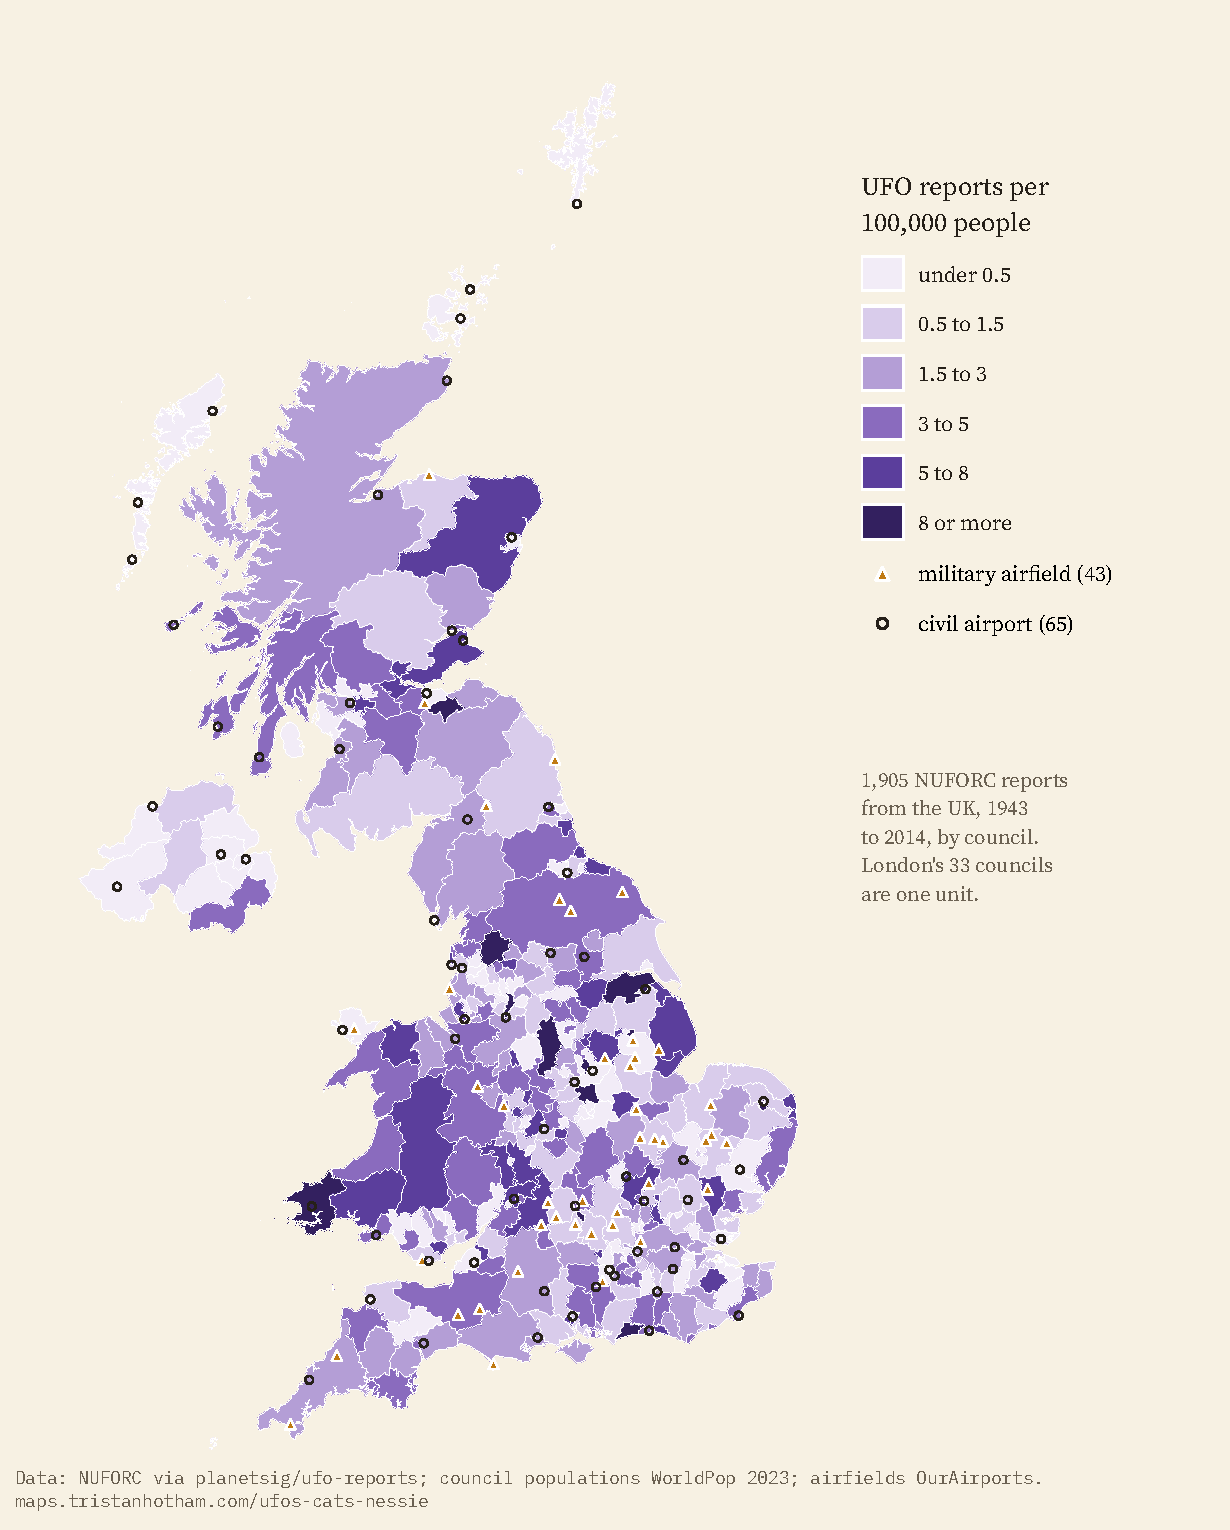
\includegraphics[width=0.72\textwidth]{f_map.pdf}\caption{UFO reports to NUFORC per 100,000 people by council unit (London merged), with military airfields (triangles) and civil airports (circles).}\label{fig:map}\end{figure}
\begin{figure}[tbp]\centering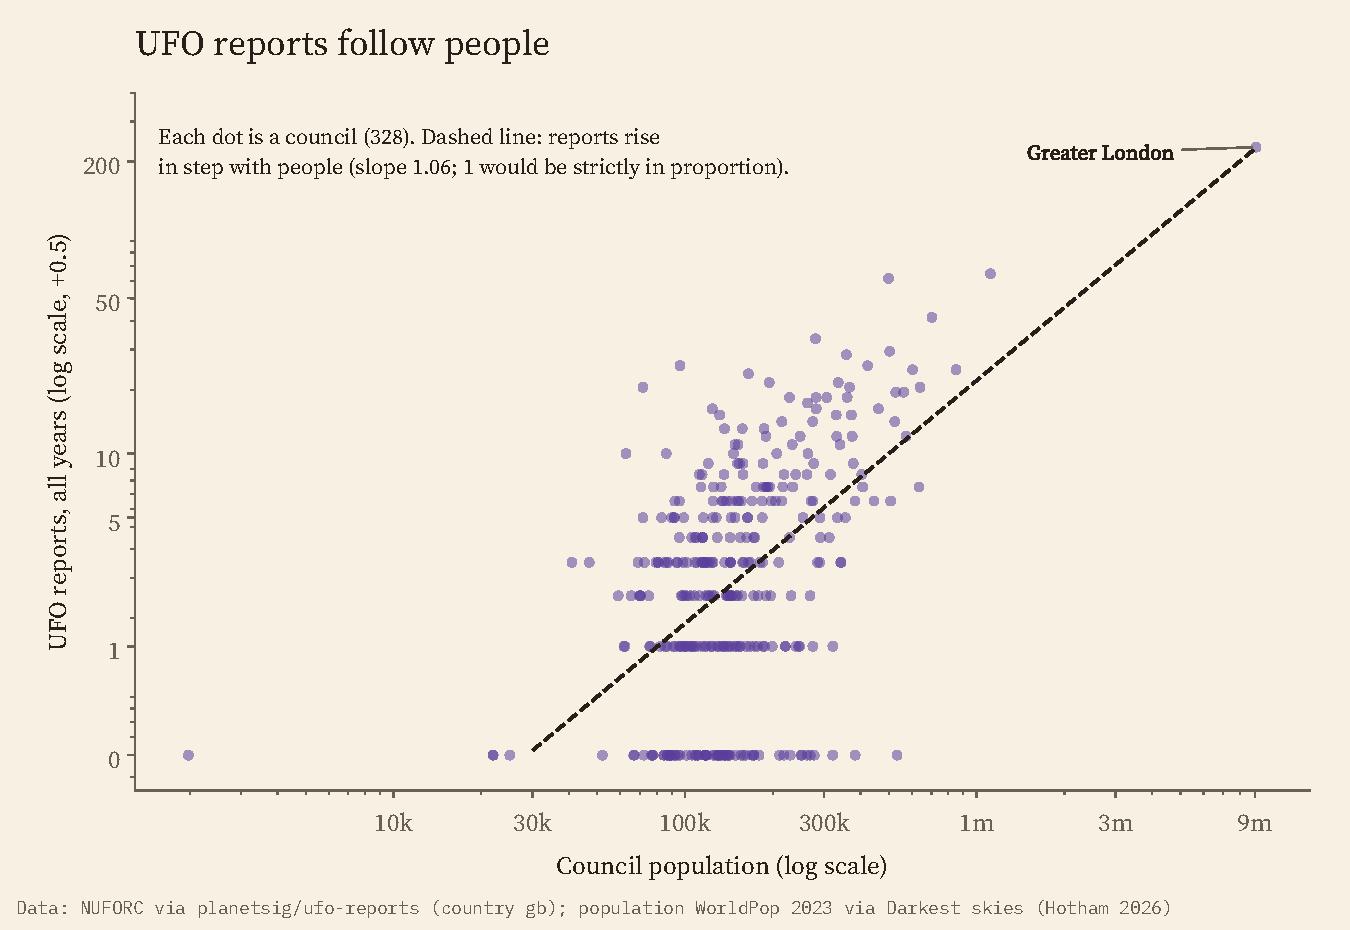
\includegraphics[width=0.8\textwidth]{f_people.pdf}\caption{Reports against population by council, log scales. The dashed line is the fitted elasticity from a model with population alone.}\label{fig:people}\end{figure}

\begin{table}[tbp]\centering\small\caption{Main model: UFO reports by council unit, negative binomial (NB2), standard errors clustered by region. Coefficients (standard errors), rate ratios with 95\% CI. N = 328 units; dispersion $\alpha$ = 0.85; reference nation England.}\label{tab:main}\begin{tabular}{lrrr}\toprule Term & Coefficient (SE) & Rate ratio [95\% CI] & $p$\\\midrule
Population (log) & 1.083 (0.082) & 2.95 [2.51, 3.47] & $<$0.001\\
Sky darkness (mag/arcsec$^2$) & -0.004 (0.072) & 1.00 [0.86, 1.15] & 0.952\\
Distance to military airfield (log km) & 0.010 (0.107) & 1.01 [0.82, 1.25] & 0.928\\
Distance to civil airport (log km) & 0.047 (0.089) & 1.05 [0.88, 1.25] & 0.596\\
Sunshine (100 hours a year) & -0.024 (0.035) & 0.98 [0.91, 1.05] & 0.498\\
Nation: Northern Ireland & -1.650 (0.249) & 0.19 [0.12, 0.31] & $<$0.001\\
Nation: Scotland & 0.144 (0.129) & 1.15 [0.90, 1.49] & 0.263\\
Nation: Wales & 0.195 (0.113) & 1.22 [0.97, 1.52] & 0.085\\
Constant & -11.236 (1.965) & & \\
\bottomrule\end{tabular}\end{table}

\subsection{When: a late-2000s peak}
UK reports to NUFORC rose from a handful a year in the early 1990s (164 in the whole decade) to 1,311 in 2000 to 2009, and peaked in 2009 with 202 reports (Figure~\ref{fig:years}). In 29 of those the reported shape was a fireball (14\%, against 4\% before 2005), which matches the Ministry of Defence's own experience of many Chinese lanterns among the reports of 2008 and 2009 \citep{tna2013}. After 2009 UK reports fell to 48 in 2013. In the interrupted series, the log ratio of UK to US reports is 62\% lower from 2010 than the 2000 to 2009 trend predicts (95\% CI 41\% to 75\% lower; N = 14 years). The placebo breaks show that this is not a clean result: the same model finds significant falls at placebo breaks in 2003 and 2004, before anything happened to the desk. The post-2009 fall is real in the data, but a fad (lanterns) ending, changes in NUFORC's own reach and the end of the official channel cannot be separated with these data.

\begin{figure}[tbp]\centering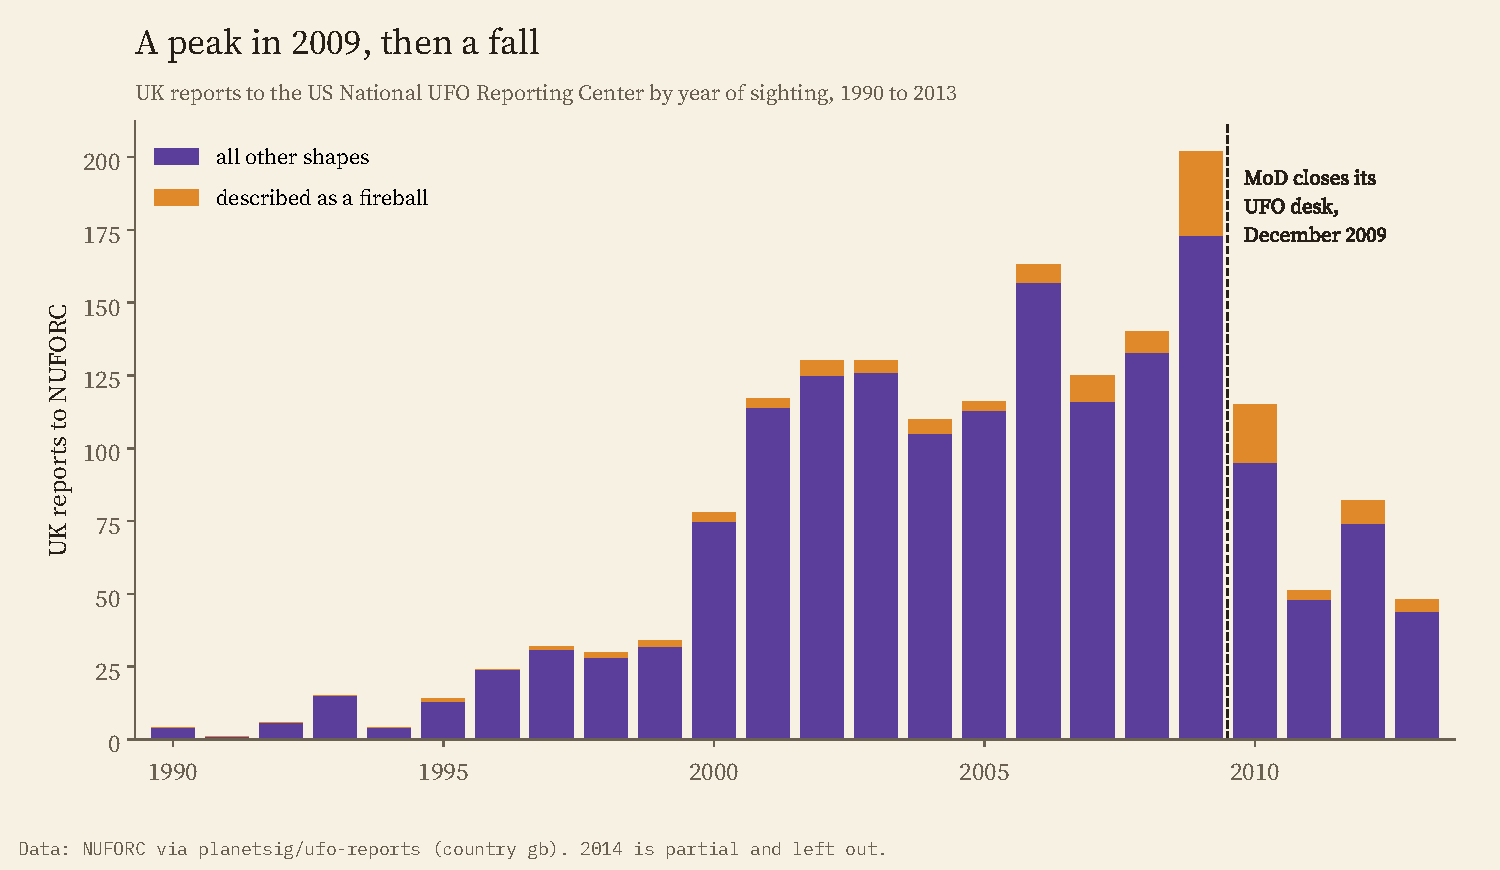
\includegraphics[width=0.85\textwidth]{f_years.pdf}\caption{UK reports to NUFORC by year of sighting, 1990 to 2013, with reports described as a fireball shown separately.}\label{fig:years}\end{figure}

\subsection{Loch Ness: born in the press}
Figure~\ref{fig:nessie} shows the register by year. Before 1933 there are a few sightings a decade. In 1933 there are 93, against 4 in the three years before, and in 1934, the year of the surgeon's photograph, 136, the most of any year in the series. The rate ratio for 1933 against the five previous years is 93 (95\% CI 38 to 293), and for 1934 6.9 (5.3 to 9.1); among 115 years with a non-zero baseline they rank 1 and 3. The later events do not stand out: 1987, the year of Operation Deepscan, has 9 sightings (ratio 0.88, CI 0.38 to 1.81, rank 56), and 2023, the year of the Quest, has 10 (ratio 0.86, CI 0.39 to 1.70, rank 57). N2 is supported for the founding events and not for later ones. One reading is that publicity created the category in 1933 and 1934 and has sustained it since without producing further surges; another is that later events were reported to a more established set of channels.

\begin{figure}[tbp]\centering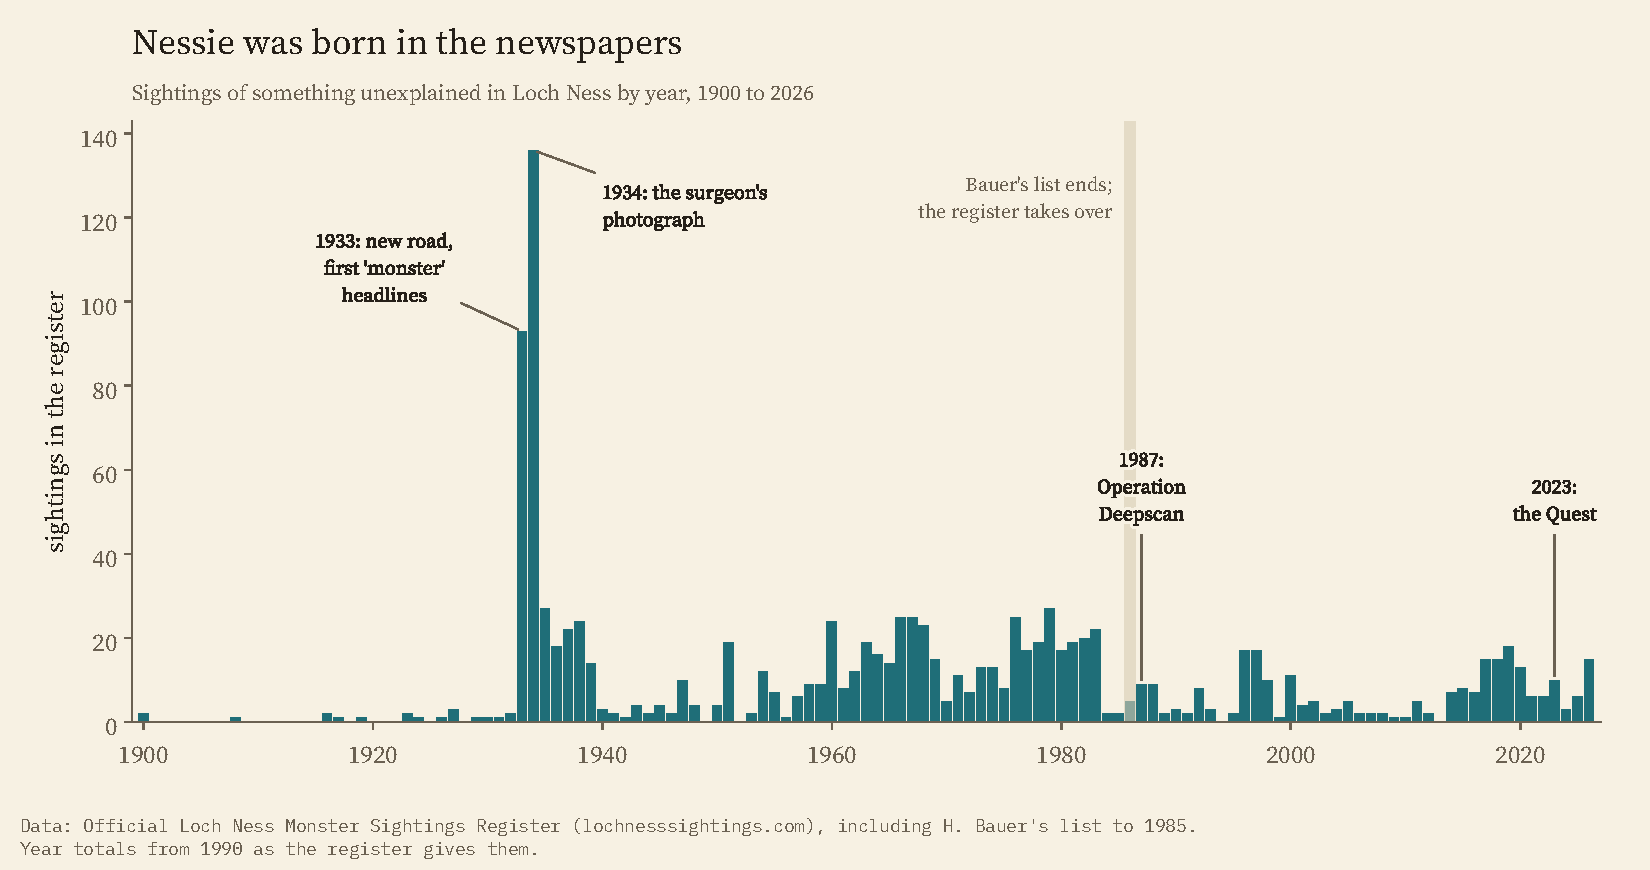
\includegraphics[width=0.9\textwidth]{f_nessie_years.pdf}\caption{Sightings in the Official Loch Ness Monster Sightings Register by year, 1900 to 2026. Bauer's list to 1985; the register's own entries from 1986, using its year totals from 1990.}\label{fig:nessie}\end{figure}

\subsection{Loch Ness: tourist hours}
Sightings per day vary strongly by month (chi-square test against a uniform rate, $p$ <0.001; N = 1,019 sightings with a month). June to August hold 48\% of sightings, against 25\% of the days, and August has 4.3 times as many sightings per day as January. Sightings per day follow day length closely (Spearman $\rho$ = 0.80, permutation $p$ = 0.002), in Bauer's list ($\rho$ = 0.75) and in the register since 1986 ($\rho$ = 0.93), and without 1933 and 1934 ($\rho$ = 0.90). The correlation with the school holiday index is weaker ($\rho$ = 0.41, $p$ = 0.10; Figure~\ref{fig:months}). The index is a crude proxy, and day length and holidays are both high in summer, so the two cannot be told apart with twelve months. Where a place is named, 46\% of the 172 sightings since 1986 with a named place are at Urquhart Castle or in Urquhart Bay, the loch's best-known visitor spot. N1 is supported.

\begin{figure}[tbp]\centering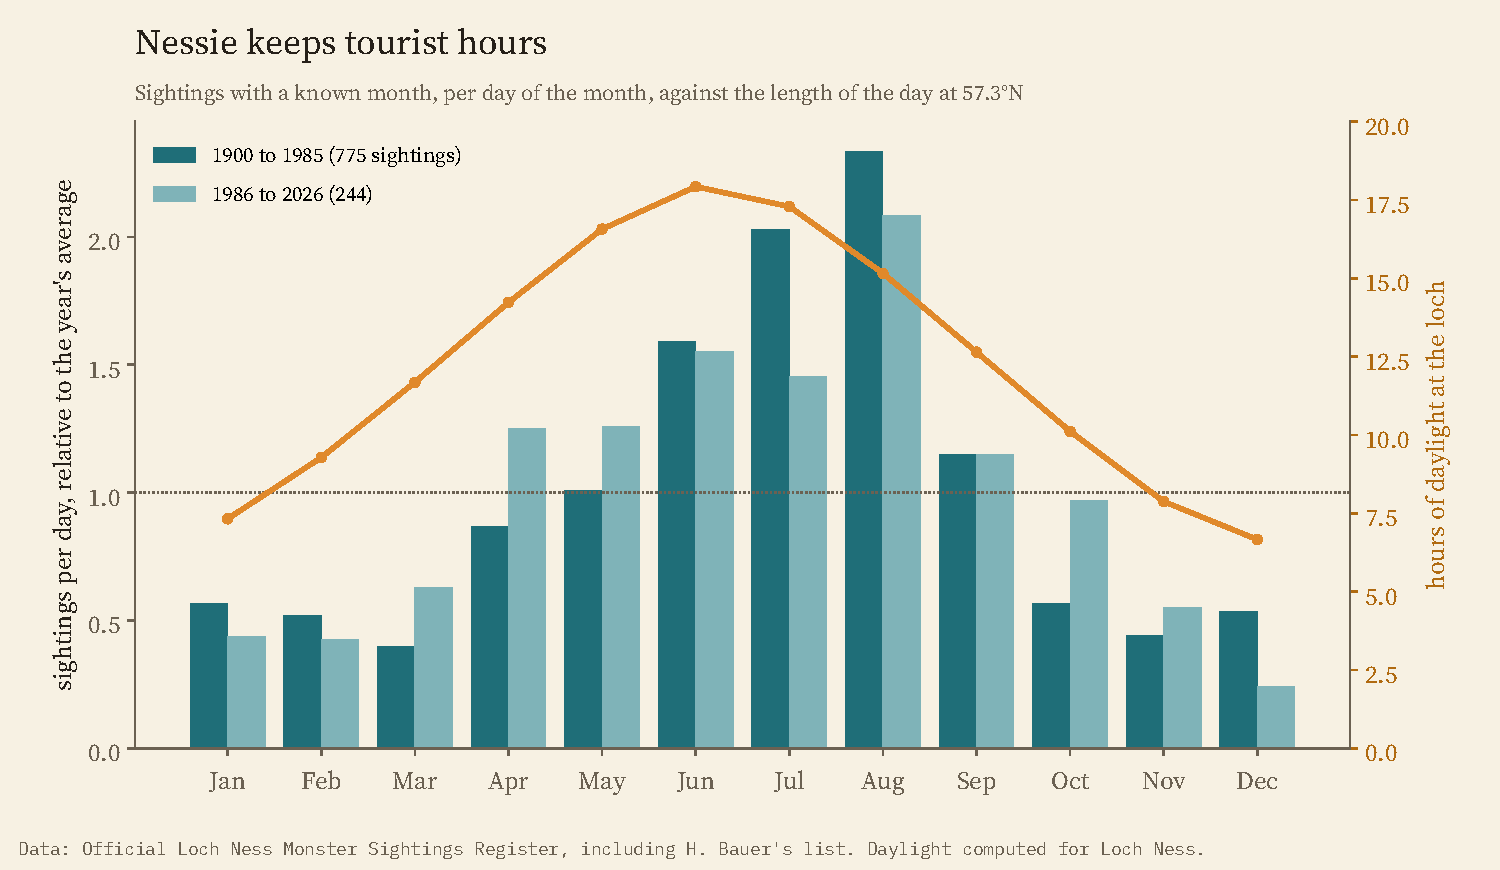
\includegraphics[width=0.85\textwidth]{f_nessie_months.pdf}\caption{Loch Ness sightings per day of each month, relative to the annual mean, for Bauer's list (1900 to 1985) and the register (1986 to 2026), with day length at 57.3$^\circ$N.}\label{fig:months}\end{figure}

\begin{table}[tbp]\centering\small\caption{Loch Ness: publicity years against the five previous years (Poisson rate ratios, exact conditional 95\% CI; rank among all years 1905 to 2025 with a non-zero baseline) and the seasonal tests (Spearman correlations of sightings per day with day length and with the school holiday index; permutation $p$).}\label{tab:nessie}\begin{tabular}{p{5.6cm}rrlrr}\toprule Year & Sightings & Prior mean & Ratio [95\% CI] & Rank & Next year\\\midrule
1933: first press reports, new road & 93 & 1.0 & 93.00 [38.46, 293.13] & 1 of 115 & 136\\
1934: the surgeon's photograph & 136 & 19.6 & 6.94 [5.31, 9.09] & 3 of 115 & 27\\
1987: Operation Deepscan & 9 & 10.2 & 0.88 [0.38, 1.81] & 56 of 115 & 9\\
2023: the Quest weekend & 10 & 11.6 & 0.86 [0.39, 1.70] & 57 of 115 & 3\\
\bottomrule\end{tabular}
\vspace{0.8em}
\begin{tabular}{p{5.6cm}rrll}\toprule Period & N & Jun to Aug & $\rho$ day length ($p$) & $\rho$ holidays ($p$)\\\midrule
1900 to 2026 & 1019 & 48\% & 0.80 (0.002) & 0.41 (0.099)\\
1900 to 1985 & 775 & 50\% & 0.75 (0.003) & 0.47 (0.062)\\
1986 to 2026 & 244 & 43\% & 0.93 (0.000) & 0.42 (0.089)\\
1900 to 2026 without 1933 and 1934 & 809 & 49\% & 0.90 (0.000) & 0.38 (0.111)\\
\bottomrule\end{tabular}\end{table}

\subsection{Big cats: the recording system}
Of the 44 forces in the batch, 20 released itemised records, 4 sent nil returns, 12 refused on cost, 4 said they held no such record, and 4 pointed to an earlier answer or did not reply (Figure~\ref{fig:cats}, Table~\ref{tab:cats}). The refusals are informative. Surrey reported that a keyword search produced more than 2,000 incidents over the period and 780 in 2018 alone, North Wales 1,160, South Wales 596 and Cheshire more than 300, in each case mostly not about big cats; Dyfed-Powys said it would have to read 65,295 calls about animals and suspicious circumstances, and Durham estimated more than a thousand incidents a year containing one of its words. Forces that released records searched with different word lists (from three words to fourteen), different fields and different filters, and some read every record by hand.

The 24 forces with counts recorded 215 reports, 207 of them in 2014 to 2018, or about 41 a year across forces covering 41\% of the UK population. Rates range from none to 0.59 reports a year per 100,000 people, highest in Hertfordshire, Suffolk and Norfolk. Against C1, rates show no clear relation to population density (Spearman $\rho$ = -0.24, $p$ = 0.25) or to the share of low-density land ($\rho$ = -0.06, $p$ = 0.80); this planned test, which counts the 4 nil returns as zeros, is null. Without the nil returns, denser forces have fewer reports per head ($\rho$ = -0.57, $p$ = 0.01; low-density land $\rho$ = 0.39, $p$ = 0.09). The answer therefore turns on whether a nil return means no reports or a search that found none, and with such different search methods neither reading can be preferred. The honest summary is that police records give at most weak evidence that big cat reports are commoner per head in less crowded force areas.

\begin{figure}[tbp]\centering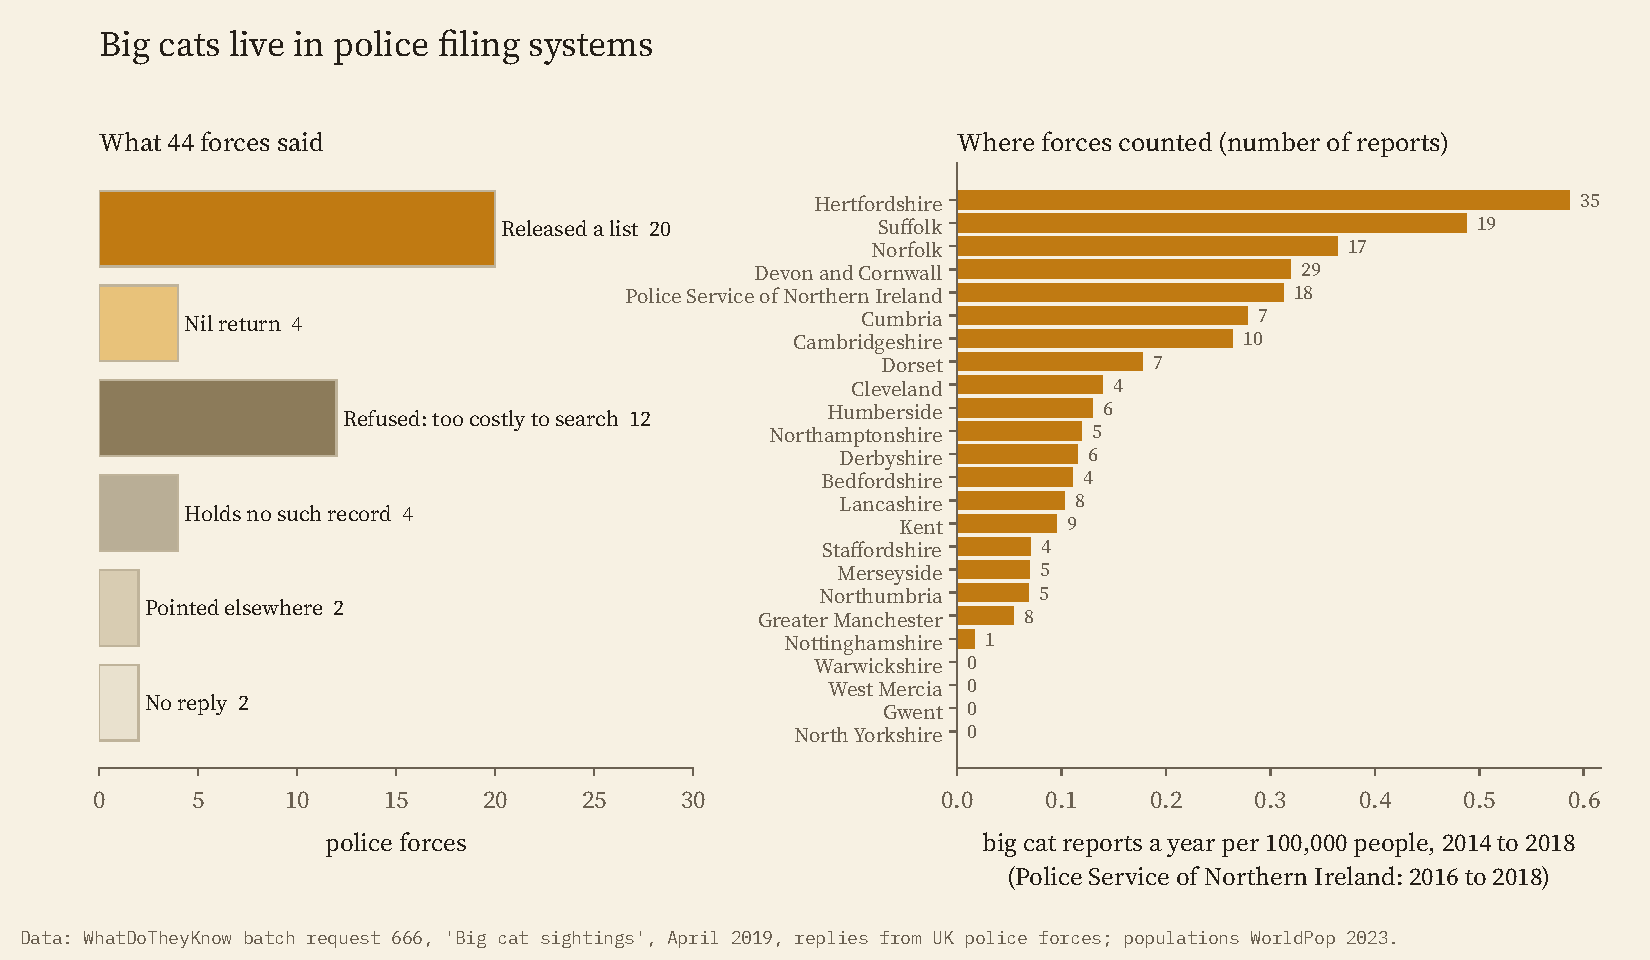
\includegraphics[width=0.95\textwidth]{f_bigcats.pdf}\caption{Replies of UK police forces to WhatDoTheyKnow batch request 666 (left) and big cat reports a year per 100,000 people, 2014 to 2018 (Police Service of Northern Ireland 2016 to 2018), in the forces that counted (right; numbers are reports).}\label{fig:cats}\end{figure}

\section{Robustness}\label{sec:robust}
Table~\ref{tab:robust} and Figure~\ref{fig:checks} show the UFO estimates under every planned check. The population elasticity stays between 1.02 and 1.10 in the alternative models listed. Across the alternative models and the three distance thresholds, no estimate shows a significant association with sky darkness, military airfields, civil airports or sunshine in the expected direction. Indicators for a military airfield within 10, 20 or 40 km give rate ratios of 0.96 (0.56 to 1.64), 1.25 (0.96 to 1.62) and 0.94 (0.73 to 1.21). Dropping each of the 12 regions in turn, the military airfield rate ratio (per unit of log distance) ranges from 0.95 to 1.09 and the sky ratio from 0.94 to 1.02; the population term is significant in 12 of 12. The negative binomial dispersion parameter is 0.85, which is why the negative binomial is the main model; the Poisson estimates agree with it.

\begin{figure}[tbp]\centering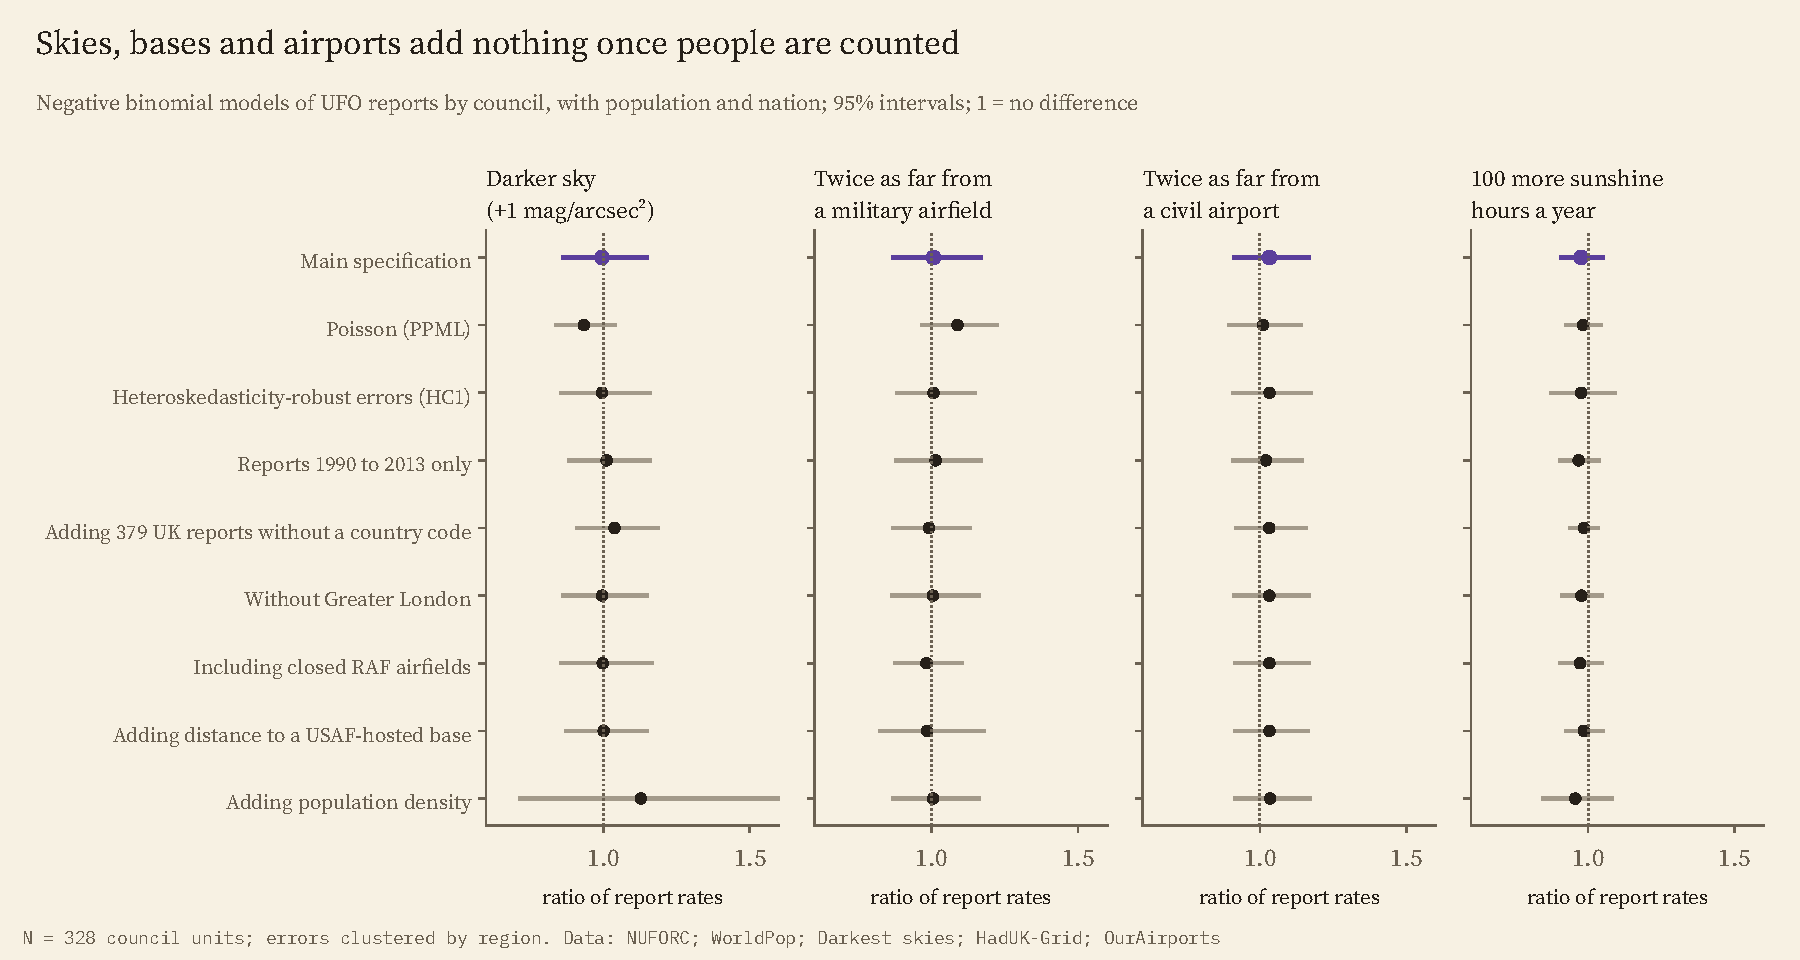
\includegraphics[width=\textwidth]{f_checks.pdf}\caption{Rate ratios (95\% CI) for the four planned covariates under each robustness check. Distances are shown for a doubling.}\label{fig:checks}\end{figure}

\begin{table}[tbp]\centering\scriptsize\caption{Robustness: the UFO model under each planned check. Population: elasticity. Other columns: rate ratios [95\% CI] per unit (sky: 1 mag/arcsec$^2$; distances: one unit of log km; sunshine: 100 hours).}\label{tab:robust}\begin{tabular}{p{4.3cm}rllllr}\toprule Model & Pop. & Sky & Military & Civil & Sunshine & N\\\midrule
Main specification & 1.08 & 1.00 [0.86, 1.15] & 1.01 [0.82, 1.25] & 1.05 [0.88, 1.25] & 0.98 [0.91, 1.05] & 328\\
Poisson (PPML) & 1.03 & 0.93 [0.84, 1.04] & 1.13 [0.96, 1.34] & 1.02 [0.85, 1.21] & 0.98 [0.93, 1.04] & 328\\
Heteroskedasticity-robust errors (HC1) & 1.08 & 1.00 [0.86, 1.16] & 1.01 [0.83, 1.22] & 1.05 [0.87, 1.26] & 0.98 [0.87, 1.09] & 328\\
Reports 1990 to 2013 only & 1.07 & 1.01 [0.88, 1.16] & 1.02 [0.83, 1.25] & 1.03 [0.87, 1.21] & 0.97 [0.90, 1.04] & 328\\
Adding 379 UK reports without a country code & 1.02 & 1.04 [0.91, 1.19] & 0.99 [0.82, 1.19] & 1.05 [0.89, 1.23] & 0.99 [0.94, 1.03] & 328\\
Without Greater London & 1.10 & 1.00 [0.86, 1.15] & 1.01 [0.81, 1.24] & 1.05 [0.88, 1.25] & 0.98 [0.91, 1.05] & 327\\
Including closed RAF airfields & 1.08 & 1.00 [0.86, 1.16] & 0.97 [0.83, 1.15] & 1.05 [0.88, 1.25] & 0.97 [0.90, 1.05] & 328\\
Adding distance to a USAF-hosted base & 1.08 & 1.00 [0.87, 1.15] & 0.98 [0.76, 1.27] & 1.05 [0.88, 1.24] & 0.99 [0.93, 1.05] & 328\\
Adding population density & 1.08 & 1.13 [0.72, 1.78] & 1.01 [0.82, 1.24] & 1.05 [0.88, 1.25] & 0.96 [0.85, 1.08] & 328\\
Military airfield within 10 km (indicator) & & & 0.96 [0.56, 1.64] & & & 328\\
Military airfield within 20 km (indicator) & & & 1.25 [0.96, 1.62] & & & 328\\
Military airfield within 40 km (indicator) & & & 0.94 [0.73, 1.21] & & & 328\\
\bottomrule\end{tabular}\end{table}

For Loch Ness, the seasonal result holds within each source (Bauer's list and the register) and without the founding years, as reported above. With the ten previous years as the baseline instead of five, 1933 and 1934 rank 1 and 3 among all years, while 1987 and 2023 rank 68 and 50 (ratios 0.60 and 1.05). The year totals I use from 1990 come from the register; using my parsed counts for 1986 on instead gives ratios of 0.88 for 1987 and 0.88 for 2023. For big cats, dropping the nil returns does change the result, as reported in Section~\ref{sec:results}: the planned test is null, the check is not.

\section{Discussion}\label{sec:disc}
Across three very different kinds of report, the pattern is the same: the distribution of reports is what one would expect from the distribution of observers, attention and record-keeping. UFO reports in the United Kingdom are found where people are, in proportion to their numbers, and not especially where skies are dark, near air bases or near airports. Loch Ness sightings were created, as a series, in the two years when the story entered the national press, and they come in the months when most people are at the loch and the days are longest. Big cat reports are held by police forces in ways that make them, for most forces, impossible to count, and the forces that can count them do so differently.

The null result for UFOs differs from the US findings of \citet{medina2023}, who found associations with sky view and with military installations. There are several reasons the two can both be right. The UK is small and densely populated, so the range of sky darkness among places where people live is narrower, and most people live near an airfield of some kind. The UK sample is also small and comes from a minority who chose to report to a US website, which may filter out exactly the casual observers whose reports respond to local conditions. And this study works at the level of councils, not small grid cells. The point-level test and the placebo were designed to catch a local effect of military airfields, and neither did.

The UFO time series is a reminder that report series respond to fashions and to channels. The fireball share of the 2009 peak matches the Ministry of Defence's experience of Chinese lanterns, and the fall after 2009 matches the end of the official channel. But the same simple model also finds significant, if smaller, falls at placebo breaks when nothing happened, so this part of the analysis supports a description, not an inference.

For Loch Ness, the founding years are so large that no statistical subtlety is needed. The seasonal profile is perhaps more telling, because it is a property of the whole record, before and after the register began, and because it follows the number of people who could be watching. Day length and holidays are proxies for watchers; the register's own guidance, like \citet{shine1988}, suggests that calm summer water, boat wakes and visitors with cameras are the mechanism. The concentration of named places at Urquhart Castle and Urquhart Bay fits the same reading.

The big cat result is the most modest and in some ways the most useful. A common claim in popular writing is that police receive many reports of big cats. The replies show that most forces cannot say. Keyword searches return hundreds or thousands of incidents about trainers, cars and leopard-print clothing, and forces refuse because reading them would cost too much. The forces that did count found a few reports a year each. Any study of big cat reports that relies on police data has to begin with the recording system.

\subsection{Limitations}
All three series are reports, not events, and each passes through selective channels. NUFORC is an American register, and its UK reports are few and self-selected; the geocoding is to towns, and London is a single point. The council covariates are measured with error, and council boundaries are coarse; associations at a finer scale could be missed, although the point-level test addresses this in part. The register's pre-1986 entries are Bauer's compression of Magin's checklist, itself compiled from books and newspapers, so the 1933 and 1934 peaks partly reflect where reports were published; that is part of the finding, not a flaw to be corrected. Optical character recognition and the parser recovered about 97\% of the register's count, and month and place are missing for some entries. The school holiday index is a typical pattern, not the calendar of each year, and visitor numbers were not available. For big cats, 20 of 44 forces gave no count, two did not reply, and the counts depend on each force's search method. The designs are observational throughout.

\section{Conclusion}\label{sec:concl}
Asked where and when people in the United Kingdom report UFOs, big cats and the Loch Ness Monster, the data give an answer that is consistent across all three: where the people are, when they are looking, when they have been told what to look for, and where someone writes it down. That does not settle any individual case. It does mean that the aggregate patterns sometimes offered as evidence for the extraordinary (more sightings here, more sightings now) are, in these data, what ordinary processes would produce.

\section*{Data availability statement}
Data and code: Zenodo DOI https://doi.org/10.5281/zenodo.24115202. The archive contains the derived datasets (UFO reports with dates, shapes and town coordinates but no text; council covariates; Loch Ness sightings with year, month and place but no names or descriptions; police force replies coded by status with yearly counts), all code, and the analysis plan. The raw sources are public: NUFORC via planetsig/ufo-reports, the register at lochnesssightings.com and the WhatDoTheyKnow threads.

\section*{AI statement}
I wrote the text, with drafting and editing assistance from Claude (Anthropic), which also helped prepare the analysis code. I reviewed and checked all text and results.

\begin{thebibliography}{99}
\bibitem[Abadie et al.(2023)]{abadie2023} Abadie, A., Athey, S., Imbens, G. W. and Wooldridge, J. M. (2023) When should you adjust standard errors for clustering? \textit{Quarterly Journal of Economics} 138(1), 1 to 35. doi:10.1093/qje/qjac038.
\bibitem[Bauer(1986)]{bauer1986} Bauer, H. H. (1986) \textit{The Enigma of Loch Ness: Making Sense of a Mystery}. Urbana and Chicago: University of Illinois Press.
\bibitem[Binns(1983)]{binns1983} Binns, R. (1983) \textit{The Loch Ness Mystery Solved}. Shepton Mallet: Open Books.
\bibitem[Blake et al.(2014)]{blake2014} Blake, M., Naish, D., Larson, G., King, C. L., Nowell, G., Sakamoto, M. and Barnett, R. (2014) Multidisciplinary investigation of a `British big cat': a lynx killed in southern England c. 1903. \textit{Historical Biology} 26(4), 441 to 448. doi:10.1080/08912963.2013.785541.
\bibitem[Boese(2002)]{boese2002} Boese, A. (2002) The surgeon's photo. \textit{The Museum of Hoaxes}, hoaxes.org/photo\_database/image/the\_surgeons\_photo. Retrieved 2026.
\bibitem[Bondarenko et al.(2025)]{bondarenko2025} Bondarenko, M. et al. (2025) \textit{The spatial distribution of population in 2015 to 2030 at 30 arc seconds}, R2025A. WorldPop, University of Southampton. doi:10.5258/SOTON/WP00845.
\bibitem[Cameron and Miller(2015)]{cameron2015} Cameron, A. C. and Miller, D. L. (2015) A practitioner's guide to cluster-robust inference. \textit{Journal of Human Resources} 50(2), 317 to 372.
\bibitem[Campbell(1991)]{campbell1991} Campbell, S. (1991) \textit{The Loch Ness Monster: The Evidence}. Aberdeen: Aberdeen University Press.
\bibitem[Clarke(2009)]{clarke2009} Clarke, D. (2009) \textit{The UFO Files: The Inside Story of Real-Life Sightings}. Kew: The National Archives.
\bibitem[Clarke(2014a)]{clarke2014} Clarke, D. (2014a) \textit{Britain's X-traordinary Files}. London: Bloomsbury.
\bibitem[Clarke(2014b)]{clarke2014b} Clarke, D. (2014b) Cat's out of the bag? Blog post, 15 December, drdavidclarke.co.uk. Retrieved 2026.
\bibitem[Clarke(2015)]{clarke2015} Clarke, D. (2015) \textit{How UFOs Conquered the World: The History of a Modern Myth}. London: Aurum Press.
\bibitem[Falchi et al.(2016)]{falchi2016} Falchi, F., Cinzano, P., Duriscoe, D., Kyba, C. C. M., Elvidge, C. D., Baugh, K., Portnov, B. A., Rybnikova, N. A. and Furgoni, R. (2016) The new world atlas of artificial night sky brightness. \textit{Science Advances} 2(6), e1600377. doi:10.1126/sciadv.1600377.
\bibitem[Hendry(1979)]{hendry1979} Hendry, A. (1979) \textit{The UFO Handbook: A Guide to Investigating, Evaluating and Reporting UFO Sightings}. Garden City, NY: Doubleday.
\bibitem[Hollis et al.(2026)]{hollis2026} Met Office, Hollis, D., McCarthy, M., Kendon, M. and Legg, T. (2026) \textit{HadUK-Grid Gridded Climate Observations on a 1km grid over the UK}, v1.3.2.ceda (1836 to 2025). NERC EDS Centre for Environmental Data Analysis. Open Government Licence v3.
\bibitem[Hotham(2026a)]{hotham2026dark} Hotham, T. (2026a) \textit{Darkest skies: where you can still see the Milky Way}. Zenodo. doi:10.5281/zenodo.23757708.
\bibitem[Hotham(2026b)]{hotham2026sun} Hotham, T. (2026b) \textit{Sun and rain: the UK's sunshine against its rainfall}. Zenodo. doi:10.5281/zenodo.23732582.
\bibitem[Hotham(2026c)]{hotham2026ghosts} Hotham, T. (2026c) \textit{Haunted, or Just Old? Britain and Ireland's reportedly haunted places against its oldest notable buildings}. Zenodo. doi:10.5281/zenodo.23691866.
\bibitem[Hotham(2026d)]{hotham2026ley} Hotham, T. (2026d) \textit{Ley Lines, Tested}. Zenodo. doi:10.5281/zenodo.23691885.
\bibitem[Inverness Courier(2023)]{courier2023} Inverness Courier (2023) Explained: what sparked the Loch Ness Monster mystery 90 years ago? inverness-courier.co.uk. Retrieved 2026.
\bibitem[Loch Ness Centre(2023)]{lochness2023} Loch Ness Centre (2023) The Quest weekend, 26 and 27 August 2023. lochness.com/the-quest-weekend. Retrieved 2026.
\bibitem[Loxton and Prothero(2013)]{loxton2013} Loxton, D. and Prothero, D. R. (2013) \textit{Abominable Science! Origins of the Yeti, Nessie, and Other Famous Cryptids}. New York: Columbia University Press.
\bibitem[Martin and Boyd(1999)]{martin1999} Martin, D. S. and Boyd, A. (1999) \textit{Nessie: The Surgeon's Photograph Exposed}. East Barnet: Martin and Boyd.
\bibitem[Medina et al.(2023)]{medina2023} Medina, R. M., Brewer, S. C. and Kirkpatrick, S. M. (2023) An environmental analysis of public UAP sightings and sky view potential. \textit{Scientific Reports} 13. doi:10.1038/s41598-023-49527-x.
\bibitem[Naish(2016)]{naish2016} Naish, D. (2016) \textit{Hunting Monsters: Cryptozoology and the Reality Behind the Myths}. London: Arcturus.
\bibitem[NUFORC(2026)]{nuforc2026} National UFO Reporting Center (2026) nuforc.org. Retrieved 2026.
\bibitem[OurAirports(2026)]{ourairports2026} OurAirports (2026) airports.csv, github.com/davidmegginson/ourairports-data. Public domain. Retrieved 2026.
\bibitem[Paxton(2009)]{paxton2009} Paxton, C. G. M. (2009) The plural of `anecdote' can be `data': statistical analysis of viewing distances in reports of unidentified large marine animals 1758 to 2000. \textit{Journal of Zoology} 279(4), 381 to 387. doi:10.1111/j.1469-7998.2009.00630.x.
\bibitem[Paxton and Naish(2019)]{paxton2019} Paxton, C. G. M. and Naish, D. (2019) Did nineteenth century marine vertebrate fossil discoveries influence sea serpent reports? \textit{Earth Sciences History} 38(1), 16 to 27. doi:10.17704/1944-6178-38.1.16.
\bibitem[planetsig(2026)]{planetsig} planetsig (2026) ufo-reports: scrubbed and geocoded NUFORC reports. github.com/planetsig/ufo-reports. Retrieved 2026.
\bibitem[Register(2026)]{register2026} The Official Loch Ness Monster Sightings Register (2026) lochnesssightings.com, including the list from Bauer (1986). Retrieved 2026.
\bibitem[Santos Silva and Tenreyro(2006)]{santos2006} Santos Silva, J. M. C. and Tenreyro, S. (2006) The log of gravity. \textit{Review of Economics and Statistics} 88(4), 641 to 658. doi:10.1162/rest.88.4.641.
\bibitem[Shine and Martin(1988)]{shine1988} Shine, A. J. and Martin, D. S. (1988) Loch Ness habitats observed by sonar and underwater television. \textit{The Scottish Naturalist}, 111 to 199.
\bibitem[The National Archives(2013)]{tna2013} The National Archives (2013) \textit{UFO Files: Highlights Guide}. Kew: The National Archives.
\bibitem[WhatDoTheyKnow(2019)]{wdtk2019} WhatDoTheyKnow (2019) Batch request 666: Big cat sightings, to UK police forces, 8 April 2019, and replies. mySociety, whatdotheyknow.com. Retrieved 2026.
\bibitem[Wikipedia contributors(2026a)]{wiki2026nessie} Wikipedia contributors (2026a) Loch Ness Monster. \textit{Wikipedia}. Retrieved 2026. CC BY-SA 4.0.
\bibitem[Wikipedia contributors(2026b)]{wiki2026wilson} Wikipedia contributors (2026b) Robert Kenneth Wilson. \textit{Wikipedia}. Retrieved 2026. CC BY-SA 4.0.
\bibitem[Williams(2015)]{williams2015} Williams, G. (2015) \textit{A Monstrous Commotion: The Mysteries of Loch Ness}. London: Orion.
\end{thebibliography}

\appendix
\section{Appendix: full tables and data construction}
\begin{table}[htbp]\centering\small\caption{UFO model dropping one region at a time (population elasticity and rate ratios).}\label{tab:lor}\begin{tabular}{lrrrrr}\toprule Region dropped & Pop. & Sky & Military & Civil & Sunshine\\\midrule
East Midlands & 1.15 & 1.00 & 1.07 & 1.00 & 0.99\\
East of England & 1.05 & 1.01 & 0.97 & 1.06 & 1.01\\
London & 1.10 & 1.00 & 1.01 & 1.05 & 0.98\\
North East & 1.08 & 1.00 & 1.00 & 1.03 & 0.97\\
North West & 1.10 & 0.98 & 1.00 & 1.06 & 0.96\\
Northern Ireland & 1.08 & 1.00 & 1.02 & 1.02 & 0.97\\
Scotland & 1.08 & 1.02 & 1.09 & 1.02 & 0.97\\
South East & 1.09 & 1.02 & 0.99 & 1.07 & 0.97\\
South West & 1.09 & 1.01 & 1.02 & 1.04 & 0.97\\
Wales & 1.05 & 0.94 & 0.95 & 1.12 & 0.99\\
West Midlands & 1.05 & 1.00 & 0.99 & 1.04 & 0.98\\
Yorkshire and The Humber & 1.10 & 0.98 & 1.01 & 1.07 & 0.97\\
\bottomrule\end{tabular}\end{table}

{\scriptsize\begin{longtable}{p{3.6cm}p{2.3cm}rrrrrrr}\caption{Every police force's reply to batch request 666, with records by year (2019 to the date of the reply) and reports a year per 100,000 people, 2014 to 2018 (Police Service of Northern Ireland 2016 to 2018).}\label{tab:cats}\\\toprule Force & Reply & 2014 & 2015 & 2016 & 2017 & 2018 & 2019 & Rate\\\midrule\endfirsthead
\toprule Force & Reply & 2014 & 2015 & 2016 & 2017 & 2018 & 2019 & Rate\\\midrule\endhead
Avon and Somerset & not held &  &  &  &  &  &  & \\
Bedfordshire & released & 0 & 1 & 1 & 2 & 0 & 0 & 0.11\\
Cambridgeshire & released & 1 & 5 & 0 & 3 & 1 & 1 & 0.26\\
Cheshire & refused (cost) &  &  &  &  &  &  & \\
City of London & not held &  &  &  &  &  &  & \\
Cleveland & released & 0 & 1 & 2 & 0 & 1 & 0 & 0.14\\
Cumbria & released & 0 & 1 & 1 & 3 & 2 & 1 & 0.28\\
Derbyshire & released & 1 & 1 & 2 & 1 & 1 & 0 & 0.12\\
Devon and Cornwall & released & 7 & 4 & 8 & 1 & 9 & 2 & 0.32\\
Dorset & released & 0 & 1 & 0 & 0 & 6 & 0 & 0.18\\
Durham & refused (cost) &  &  &  &  &  &  & \\
Dyfed-Powys & refused (cost) &  &  &  &  &  &  & \\
Essex & refused (cost) &  &  &  &  &  &  & \\
Gloucestershire & refused (cost) &  &  &  &  &  &  & \\
Greater Manchester & released & 3 & 0 & 2 & 1 & 2 & 0 & 0.05\\
Gwent & nil return & 0 & 0 & 0 & 0 & 0 & 0 & 0.00\\
Hampshire & refused (cost) &  &  &  &  &  &  & \\
Hertfordshire & released & 7 & 5 & 5 & 13 & 5 & 2 & 0.59\\
Humberside & released & 2 & 0 & 3 & 0 & 1 & 0 & 0.13\\
Kent & released & 4 & 1 & 3 & 1 & 0 & 0 & 0.10\\
Lancashire & released & 1 & 1 & 2 & 3 & 1 & 0 & 0.10\\
Leicestershire & no reply &  &  &  &  &  &  & \\
Merseyside & released & 3 & 0 & 0 & 1 & 1 & 0 & 0.07\\
Metropolitan Police & not held &  &  &  &  &  &  & \\
Norfolk & released & 5 & 4 & 3 & 1 & 4 & 0 & 0.36\\
North Wales & refused (cost) &  &  &  &  &  &  & \\
North Yorkshire & nil return & 0 & 0 & 0 & 0 & 0 & 0 & 0.00\\
Northamptonshire & released & 1 & 0 & 1 & 2 & 1 & 0 & 0.12\\
Northumbria & released & 1 & 2 & 0 & 1 & 1 & 1 & 0.07\\
Nottinghamshire & released & 0 & 1 & 0 & 0 & 0 & 0 & 0.02\\
Police Scotland & refused (cost) &  &  &  &  &  &  & \\
Police Service of Northern Ireland & released & 0 & 0 & 1 & 11 & 6 & 1 & 0.31\\
South Wales & refused (cost) &  &  &  &  &  &  & \\
South Yorkshire & pointed elsewhere &  &  &  &  &  &  & \\
Staffordshire & released & 0 & 2 & 1 & 1 & 0 & 0 & 0.07\\
Suffolk & released & 4 & 3 & 5 & 3 & 4 & 0 & 0.49\\
Surrey & refused (cost) &  &  &  &  &  &  & \\
Sussex & no reply &  &  &  &  &  &  & \\
Thames Valley & refused (cost) &  &  &  &  &  &  & \\
Warwickshire & nil return & 0 & 0 & 0 & 0 & 0 & 0 & 0.00\\
West Mercia & nil return & 0 & 0 & 0 & 0 & 0 & 0 & 0.00\\
West Midlands & refused (cost) &  &  &  &  &  &  & \\
West Yorkshire & pointed elsewhere &  &  &  &  &  &  & \\
Wiltshire & not held &  &  &  &  &  &  & \\
\bottomrule\end{longtable}}

Table~\ref{tab:lor} gives the leave-one-region-out estimates and Table~\ref{tab:cats} every police force's reply. \textbf{Decisions made by hand.} The London merge, the airfield definitions (including Alconbury, listed by OurAirports as closed for flying but a United States Air Force site throughout the period, and excluding Croughton, which has no airfield) and the police force areas were fixed before outcomes were examined. In Cleveland's list, three records of domestic black cats were removed. Durham refused on cost but gave one record as a gesture; it is coded as a refusal and its record is not used in rates. Two Bauer pages were checked entry by entry against the scans.

\textbf{Software.} Python 3 with pandas, numpy, shapely, pyproj, statsmodels, scipy, matplotlib and Pillow; Tesseract for optical character recognition; xelatex. All code is in the data and code archive.

\end{document}
